\documentclass[12pt,a4paper]{ctexart}
\usepackage[a4paper,top=25mm,bottom=25mm,left=25mm,right=25mm,headheight=15pt]{geometry}
\usepackage{amsmath,amssymb,bm,booktabs,longtable,array,tabularx,multirow}
\usepackage{graphicx,float,subcaption,xcolor,hyperref,fancyhdr,enumitem}
\usepackage{setspace}
\graphicspath{{figures/}}
\hypersetup{colorlinks=true,linkcolor=black,citecolor=black,urlcolor=blue}
\setstretch{1.30}
\setlength{\parindent}{2em}
\setlength{\parskip}{0pt}
\setlist{nosep,leftmargin=2em}
\pagestyle{fancy}
\fancyhf{}
\lhead{2026年高教社杯全国大学生数学建模竞赛}
\rhead{A题：药材的烘干问题}
\cfoot{\thepage}
\newcommand{\QThreeDryHours}{57.5303}
\newcommand{\QFourDryHours}{52.6776}
\newcommand{\AppendixFourFixedHours}{129.9873}
\newcommand{\NoCoordinateCaseHours}{51.1141}
\newcommand{\ShrinkReduction}{59.47\%}
\newcommand{\AppendixIncrease}{125.95\%}
\newcommand{\OmitCoordinateDifference}{-2.97\%}
\newcommand{\NetReduction}{8.44\%}
\newcommand{\StableStartHours}{2.050}
\newcommand{\PlateauTemperature}{50.0049}
\newcommand{\PlateauMoisture}{0.049994}
\newcommand{\QFourDryRadius}{1.2000}
\newcommand{\ConservationError}{1.61e-15}
\newcommand{\EquilibriumError}{2.06e-11}
\newcommand{\QThreeGridChange}{0.092\%}
\newcommand{\QFourGridChange}{0.045\%}
\newcommand{\QFourTimeChange}{0.00148\%}
\newcommand{\QOneMoistureProfileError}{8.69e-05}
\newcommand{\QTwoMoistureProfileError}{2.92e-06}


\title{\vspace{-2.2em}\bfseries 基于热质耦合与移动边界的药材烘干模型}
\author{}
\date{}

\begin{document}
\maketitle
\vspace{-4em}

\begin{abstract}
针对圆柱形中药材热风烘干过程，建立一维径向非线性热质耦合模型。以附件1的烘房温度和水分浓度作为时变Robin边界，分别代入附录2--4的物性关系；在问题1--3中对物理径向坐标 $r$ 划分，在问题4中先令 $\xi=r/R(t)$、再对相对坐标 $\xi$ 划分，并对半节点之间的径向区间作守恒积分。空间离散采用柱坐标有限体积通量平衡，时间离散采用后向欧拉启动、二阶后向差分推进，并在每个时间层用Picard迭代更新温度、含水率及物性。问题4由附件2分段线性构造动态半径，主模型保留坐标变换产生的几何输运项。计算网格与题目规定的输出网格分离：问题1--3使用641个径向节点，问题4使用321个相对坐标节点，结果再采样至题目规定的位置。

数值结果表明，1800 s时中心与表面温度分别为33.5753 $^\circ$C和36.7856 $^\circ$C，含水率分别为2.5500和1.5102 kg/kg；3 h时中心温度为49.8495 $^\circ$C，中心含水率为1.7662 kg/kg。以全场最大含水率首次不超过0.15 kg/kg为终止条件，固定半径、附录3物性下的烘干时长为\QThreeDryHours\ h；考虑附录4物性和实测收缩后为\QFourDryHours\ h，此时半径约\QFourDryRadius\ cm。封闭系统守恒误差为\ConservationError，空间、时间收敛检验均通过；省略问题4的几何输运项会把时长低估约2.97\%。模型能够解释中心最后达标及收缩缩短扩散路径的规律，并生成题目要求的四个完整结果文件。

\textbf{关键词：}药材烘干；热质耦合；有限体积法；BDF；移动边界
\end{abstract}

\section{问题分析}
\subsection{任务分解}
药材长25 cm、初始半径2 cm，可近似为轴对称长圆柱。问题1要求求出前30 min的温度场和含水率场；问题2将物性改为温度、含水率的函数并计算前3 h；问题3沿用问题2模型，确定所有位置含水率均不高于0.15 kg/kg的时刻；问题4再加入附件2给出的半径收缩和附录4物性，重新计算干燥终点。四问的物理核心相同，适合建立统一求解器，仅切换物性、半径和终止条件。

\subsection{主要困难}
第一，柱坐标方程含 $1/r$，圆心不能直接套用普通差分；第二，$D(C,T)$ 呈指数变化，低含水率区会形成薄扩散层，离散系统非线性且刚性；第三，问题4的区域 $0\le r\le R(t)$ 随时间变化，固定物理坐标节点会逐渐退出药材。为保证边界通量与内部通量符号一致，空间上采用守恒型有限体积法；为处理收缩域，采用 $\xi=r/R(t)$ 将其映射到固定区间。

\subsection{求解路线与数据处理}
附件1共有241个采样点，时间为0--14400 s、间隔60 s。在测量区间内对烘房温度 $T_a(t)$ 和水分浓度 $C_a(t)$ 作分段线性插值；4 h后取9000 s以后数据均值
\[
T_a^*=\PlateauTemperature\ ^\circ\mathrm C,\qquad C_a^*=\PlateauMoisture.
\]
按温度偏差小于0.5 $^\circ$C、水分浓度偏差小于 $10^{-3}$ 且持续30 min的判据，稳定段约从\StableStartHours\ h开始。附件2共有145个半径点，覆盖0--72 h，问题4用分段线性函数 $R(t)$ 及各段斜率 $\dot R(t)$。边界与半径变化见图\ref{fig:boundary}。
\begin{figure}[H]
\centering
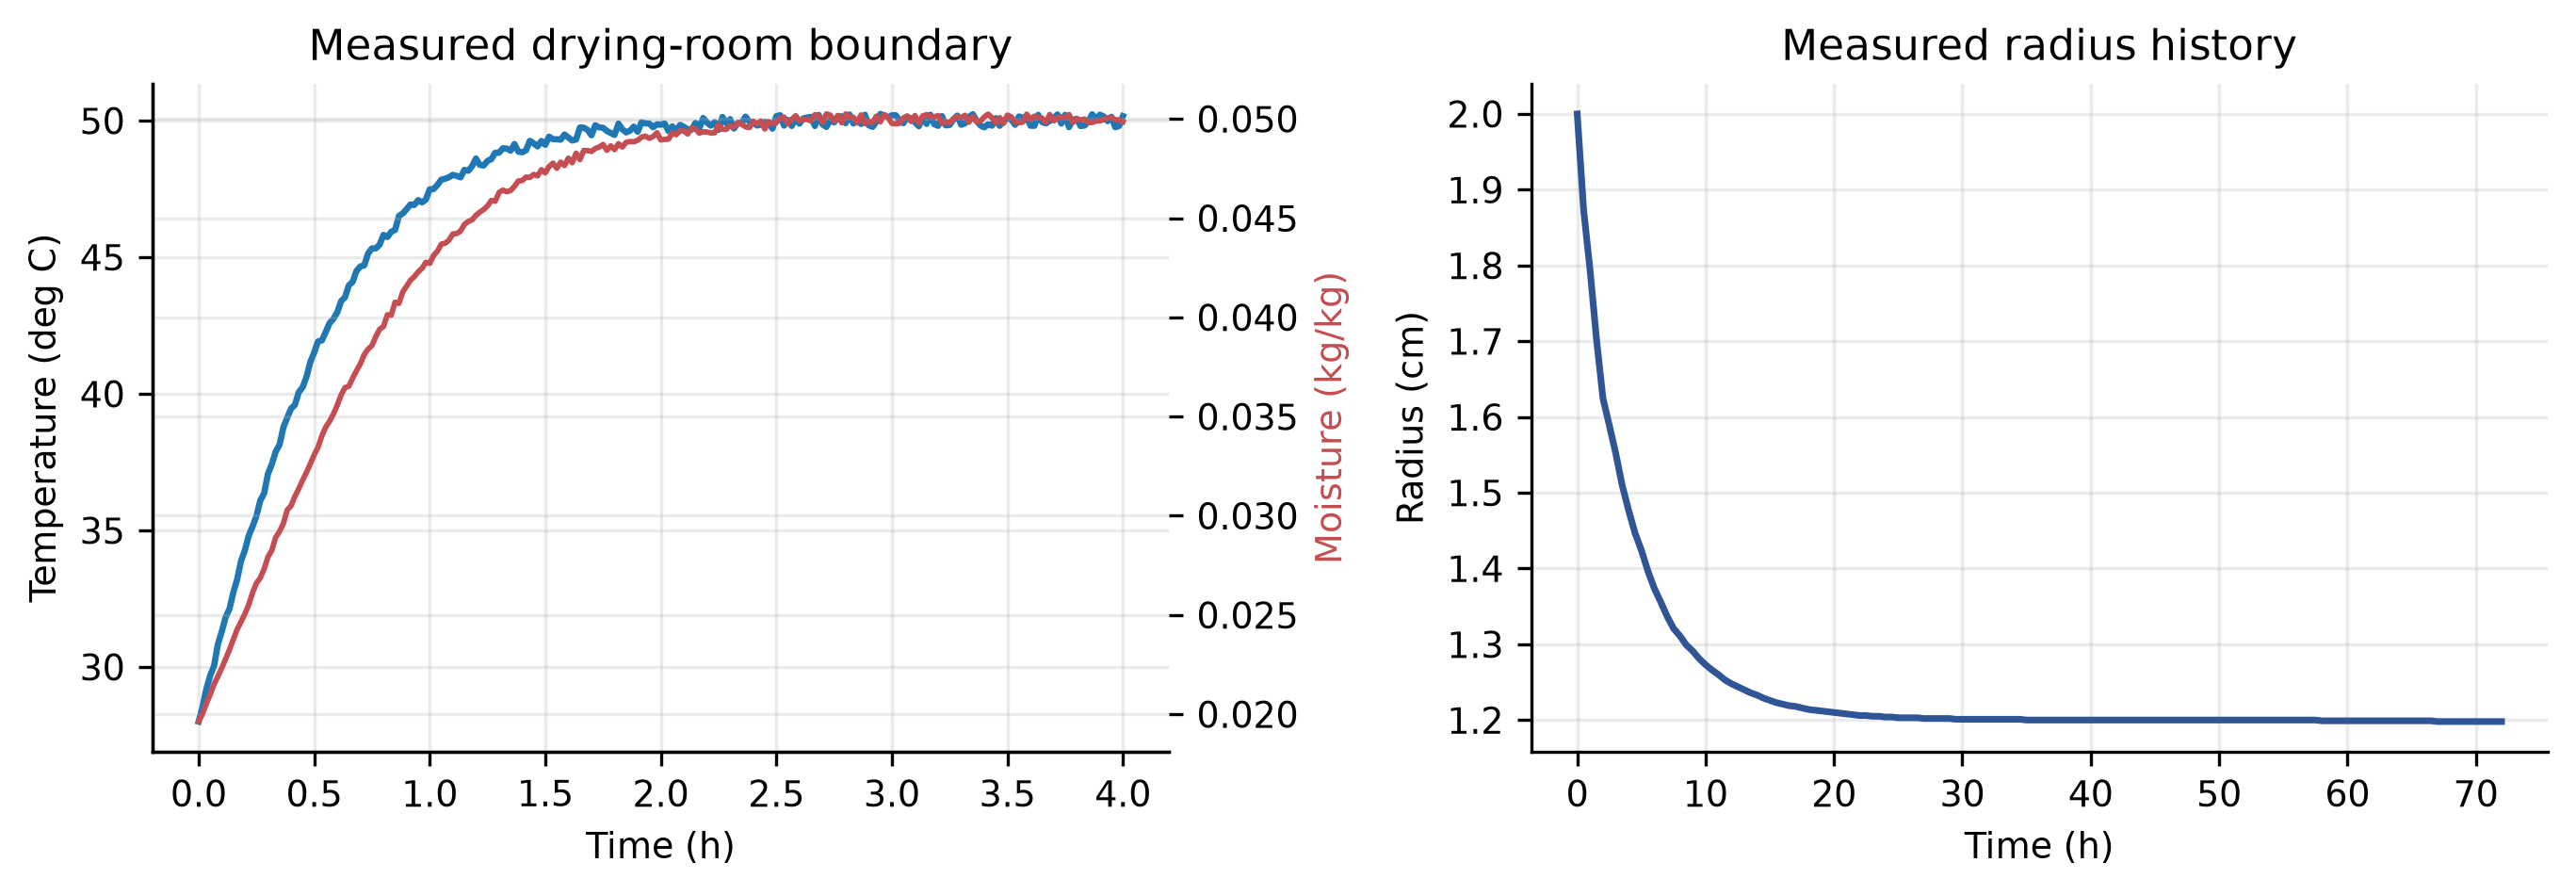
\includegraphics[width=0.96\textwidth]{boundary_data.png}
\caption{烘房边界与药材半径的附件数据}\label{fig:boundary}
\end{figure}

\section{模型假设}
\begin{enumerate}
  \item 药材为各向同性、轴对称的均匀圆柱；长度远大于半径，忽略端面附近的轴向温度和水分梯度。
  \item 药材内部仅考虑导热与有效水分扩散；蒸发潜热、体积热源、化学反应和辐射换热并入经验参数误差。
  \item 初始温度和干基含水率均匀，分别为301.15 K和2.55 kg/kg。
  \item 题目仅在附录2给出问题1的换热、传质系数，问题2--4沿用 $h=25\ \mathrm{W/(m^2K)}$ 与 $h_m=8\times10^{-7}\ \mathrm{m/s}$。
  \item 附件1测量区间内作分段线性插值；烘房稳定后，环境温度和水分浓度取后段测量均值。
  \item 问题4的收缩在径向均匀发生，$R(t)$ 由附件2分段线性插值；长度变化忽略。$T(\xi,t),C(\xi,t)$ 表示在随径向网格运动的相对坐标下观察到的状态。
\end{enumerate}

\section{符号说明}
\begin{table}[H]
\centering
\caption{主要符号及有限体积下标约定}
\begin{tabularx}{\textwidth}{cXc}
\toprule
符号 & 含义 & 单位\\
\midrule
$r$ & 问题1--3的物理径向坐标，$0\le r\le R$ & m\\
$R,R(t)$ & 固定半径、问题4的时变半径 & m\\
$\xi$ & 问题4的相对坐标，$\xi=r/R(t)\in[0,1]$ & --\\
$T(r,t),C(r,t)$ & 药材温度、干基含水率 & K，kg/kg\\
$T_a(t),C_a(t)$ & 烘房温度、烘房水分浓度 & K，kg/kg\\
$\rho,c_p,k,D$ & 密度、比热容、导热系数、有效扩散系数 & 见题面\\
$h,h_m$ & 对流换热系数、对流传质系数 & W/(m$^2$K)，m/s\\
$r_i,r_{i\pm1/2}$ & $r$ 坐标节点及其左右半节点 & m\\
$\xi_i,\xi_{i\pm1/2}$ & $\xi$ 坐标节点及其左右半节点 & --\\
$T_i,C_i$ & 节点 $i$ 处温度、含水率的离散值 & K，kg/kg\\
$\Gamma_{i+1/2}$ & 界面传递系数，热场取 $k$，湿场取 $D$ & W/(mK)或m$^2$/s\\
$\omega_i^{r},\omega_i^{\xi}$ & 由相邻半节点区间积分得到的径向几何权重 & m$^2$，--\\
$N,\Delta r,\Delta\xi$ & 区间数及 $r$、$\xi$ 的网格间距 & --，m，--\\
$t_d$ & 全场含水率达到阈值的时间 & h\\
\bottomrule
\end{tabularx}
\end{table}

\section{模型建立}
\subsection{固定半径热质耦合控制方程的物理推导与建立}
药材热风烘干过程本质上是热量由烘房热风向药材内部传导、水分由药材内部向表面迁移蒸发的耦合非定常传递过程，二者均严格遵循“微元内物理量的时间积累率等于各边界面通量的净流入率”之守恒原理。

\subsubsection{直角坐标系下的守恒定律与本构方程}
药材内部的热量传递与水分迁移具有高度的物理对偶性与数学对称性，二者均由梯度驱动的通量本构关系和微元守恒原理共同确定。

首先，在通量本构层面，各向同性介质内的热流密度矢量 $\mathbf{q}$ 与水分扩散通量矢量 $\mathbf{J}$ 分别服从 Fourier 导热定律与 Fick 扩散第一定律：
\begin{align}
\mathbf{q} &= -k\nabla T,\label{eq:fourier}\\
\mathbf{J} &= -D\nabla C,\label{eq:fick}
\end{align}
其中 $k$ 为介质的导热系数，$D$ 为水分有效扩散系数，$T$ 为绝对温度，$C$ 为干基含水率；负号表示热量自高温区向低温区传导、水分自高浓度区向低浓度区迁移。

其次，在微元守恒层面，由连续介质力学原理，微元控制体内物理量的时间积累率严格等于通过控制体各界面的净流入通量。忽略内部反应与相变内热源，热能与水分分别满足能量守恒定律与质量守恒定律：
\begin{align}
\rho c_p\frac{\partial T}{\partial t} &= -\nabla\cdot\mathbf{q},\label{eq:cons_energy}\\
\frac{\partial C}{\partial t} &= -\nabla\cdot\mathbf{J},\label{eq:cons_mass}
\end{align}
其中 $\rho$ 为药材密度，$c_p$ 为定压比热容。

将 Fourier 导热定律式\eqref{eq:fourier}与能量守恒方程\eqref{eq:cons_energy}联立，Fick 扩散定律式\eqref{eq:fick}与质量守恒方程\eqref{eq:cons_mass}联立，分别得到包含 $\nabla$ 算子的控制方程：
\begin{align}
\rho c_p\frac{\partial T}{\partial t} &= \nabla\cdot(k\nabla T),\label{eq:div_heat}\\
\frac{\partial C}{\partial t} &= \nabla\cdot(D\nabla C).\label{eq:div_mass}
\end{align}
在三维直角坐标系 $(x,y,z)$ 下展开上述方程，即可导出直角坐标系下的三维热质耦合控制偏微分方程：
\begin{align}
\rho c_p\frac{\partial T}{\partial t}
&=\frac{\partial}{\partial x}\left(k\frac{\partial T}{\partial x}\right)
+\frac{\partial}{\partial y}\left(k\frac{\partial T}{\partial y}\right)
+\frac{\partial}{\partial z}\left(k\frac{\partial T}{\partial z}\right),\label{eq:cartesian_heat}\\
\frac{\partial C}{\partial t}
&=\frac{\partial}{\partial x}\left(D\frac{\partial C}{\partial x}\right)
+\frac{\partial}{\partial y}\left(D\frac{\partial C}{\partial y}\right)
+\frac{\partial}{\partial z}\left(D\frac{\partial C}{\partial z}\right).\label{eq:cartesian_mass}
\end{align}

\subsubsection{直角坐标系到柱坐标系的变换推导与控制方程建立}
由于中药材外观呈规则圆柱体形态，在直角坐标系下边界几何曲面（$x^2+y^2=R^2$）描述较为繁琐，且难以直接施加表面径向对流与扩散边界条件。因此，必须将式\eqref{eq:cartesian_heat}、\eqref{eq:cartesian_mass}所示的控制方程由直角坐标系 $(x,y,z)$ 变换至正交柱坐标系 $(r,\theta,z)$。

直角坐标与柱坐标之间的正变换与逆变换关系为：
\begin{equation}
\begin{cases}
x = r\cos\theta,\\
y = r\sin\theta,\\
z = z,
\end{cases}
\iff
\begin{cases}
r = \sqrt{x^2+y^2},\\[4pt]
\theta = \arctan(y/x),\\[4pt]
z = z.
\end{cases}
\end{equation}
根据多元微积分复合函数的链式求导法则，空间一阶偏导数算子与柱坐标偏导数算子的对应变换关系可紧凑地表示为矩阵形式：
\begin{equation}
\begin{bmatrix}
\dfrac{\partial}{\partial x} \\[10pt]
\dfrac{\partial}{\partial y} \\[10pt]
\dfrac{\partial}{\partial z}
\end{bmatrix}
=
\begin{bmatrix}
\dfrac{\partial r}{\partial x} & \dfrac{\partial\theta}{\partial x} & 0 \\[10pt]
\dfrac{\partial r}{\partial y} & \dfrac{\partial\theta}{\partial y} & 0 \\[10pt]
0 & 0 & 1
\end{bmatrix}
\begin{bmatrix}
\dfrac{\partial}{\partial r} \\[10pt]
\dfrac{\partial}{\partial\theta} \\[10pt]
\dfrac{\partial}{\partial z}
\end{bmatrix}
=
\begin{bmatrix}
\cos\theta & -\dfrac{\sin\theta}{r} & 0 \\[10pt]
\sin\theta & \dfrac{\cos\theta}{r} & 0 \\[10pt]
0 & 0 & 1
\end{bmatrix}
\begin{bmatrix}
\dfrac{\partial}{\partial r} \\[10pt]
\dfrac{\partial}{\partial\theta} \\[10pt]
\dfrac{\partial}{\partial z}
\end{bmatrix}.\label{eq:jacobi_transform}
\end{equation}
微元线元弧长平方 $ds^2=dx^2+dy^2+dz^2=dr^2+r^2d\theta^2+dz^2$，给出柱坐标系下的三个正交 Lamé 尺度因子分别为 $h_r=1, h_\theta=r, h_z=1$。据此，柱坐标正交基底 $(\mathbf{e}_r,\mathbf{e}_\theta,\mathbf{e}_z)$ 下的梯度算子 $\nabla$ 表示为：
\begin{align}
\nabla &= \frac{1}{h_r}\frac{\partial}{\partial r}\mathbf{e}_r + \frac{1}{h_\theta}\frac{\partial}{\partial\theta}\mathbf{e}_\theta + \frac{1}{h_z}\frac{\partial}{\partial z}\mathbf{e}_z \notag\\
&= \mathbf{e}_r\frac{\partial}{\partial r} + \mathbf{e}_\theta\frac1r\frac{\partial}{\partial\theta} + \mathbf{e}_z\frac{\partial}{\partial z}.\label{eq:grad_cyl}
\end{align}
对于任意矢量场 $\mathbf{A}=A_r\mathbf{e}_r+A_\theta\mathbf{e}_\theta+A_z\mathbf{e}_z$，由正交曲线坐标系下的散度算子公式：
\begin{align}
\nabla\cdot\mathbf{A} &= \frac{1}{h_rh_\theta h_z}\left[\frac{\partial}{\partial r}(h_\theta h_zA_r) + \frac{\partial}{\partial\theta}(h_rh_zA_\theta) + \frac{\partial}{\partial z}(h_rh_\theta A_z)\right] \notag\\
&= \frac1r\frac{\partial}{\partial r}(rA_r) + \frac1r\frac{\partial A_\theta}{\partial\theta} + \frac{\partial A_z}{\partial z}.\label{eq:div_cyl}
\end{align}
将传热通量矢量 $\mathbf{A}=k\nabla T$ 与传质通量矢量 $\mathbf{A}=D\nabla C$ 在柱坐标下的正交分量分别代入上述散度展开式中：
\begin{align}
\nabla\cdot(k\nabla T) &= \frac1r\frac{\partial}{\partial r}\left(rk\frac{\partial T}{\partial r}\right) + \frac1r\frac{\partial}{\partial\theta}\left(\frac{k}{r}\frac{\partial T}{\partial\theta}\right) + \frac{\partial}{\partial z}\left(k\frac{\partial T}{\partial z}\right)\notag\\
&= \frac1r\frac{\partial}{\partial r}\left(rk\frac{\partial T}{\partial r}\right) + \frac{1}{r^2}\frac{\partial}{\partial\theta}\left(k\frac{\partial T}{\partial\theta}\right) + \frac{\partial}{\partial z}\left(k\frac{\partial T}{\partial z}\right),\label{eq:div_heat_cyl}\\[10pt]
\nabla\cdot(D\nabla C) &= \frac1r\frac{\partial}{\partial r}\left(rD\frac{\partial C}{\partial r}\right) + \frac1r\frac{\partial}{\partial\theta}\left(\frac{D}{r}\frac{\partial C}{\partial\theta}\right) + \frac{\partial}{\partial z}\left(D\frac{\partial C}{\partial z}\right)\notag\\
&= \frac1r\frac{\partial}{\partial r}\left(rD\frac{\partial C}{\partial r}\right) + \frac{1}{r^2}\frac{\partial}{\partial\theta}\left(D\frac{\partial C}{\partial\theta}\right) + \frac{\partial}{\partial z}\left(D\frac{\partial C}{\partial z}\right).\label{eq:div_mass_cyl}
\end{align}
由此推导并在推导之后给出柱坐标系下的三维具体展开形式：
\begin{align}
\rho c_p\frac{\partial T}{\partial t}
&=\frac1r\frac{\partial}{\partial r}\left(rk\frac{\partial T}{\partial r}\right)
+\frac{1}{r^2}\frac{\partial}{\partial\theta}\left(k\frac{\partial T}{\partial\theta}\right)
+\frac{\partial}{\partial z}\left(k\frac{\partial T}{\partial z}\right),\label{eq:cyl_heat}\\[10pt]
\frac{\partial C}{\partial t}
&=\frac1r\frac{\partial}{\partial r}\left(rD\frac{\partial C}{\partial r}\right)
+\frac{1}{r^2}\frac{\partial}{\partial\theta}\left(D\frac{\partial C}{\partial\theta}\right)
+\frac{\partial}{\partial z}\left(D\frac{\partial C}{\partial z}\right).\label{eq:cyl_mass}
\end{align}

\subsubsection{柱坐标扩散方程的简化}
式\eqref{eq:cyl_heat}与式\eqref{eq:cyl_mass}给出了完整的三维柱坐标热质耦合偏微分方程。为提高数值求解效率并抓住主导物理过程，结合烘干实验工况与药材几何参数，将三维控制方程简化为一维径向方程。支撑该降维简化的物理与几何证据分条陈列如下：
\begin{enumerate}[label=(\arabic*)]
  \item \textbf{周向均匀性与旋转对称性证据}：
  药材外观呈规则圆柱体，关于中心旋转轴具备严格的几何旋转对称性。烘房内热风流动平稳且均匀掠过圆柱周向外表面，环境温度 $T_a(t)$、环境水分浓度 $C_a(t)$ 以及表面对流换热与传质系数 $h, h_m$ 均不依赖于周向角 $\theta$。同时，烘干初始时刻药材内部温度（$28^\circ\text{C}$）与含水率（$2.55\text{ kg/kg}$）在全截面上均匀分布，不存在周向驱动力或扰动。因此，温度场和水分场满足周向各向同性，即 $\frac{\partial T}{\partial\theta}=0$、$\frac{\partial C}{\partial\theta}=0$，角向一阶与二阶导数项严格为零。

  \item \textbf{大长径比与大面积比几何证据}：
  药材实测几何尺寸为长度 $L=25\text{ cm}$，初始半径 $R_0=2\text{ cm}$（直径 $2R_0=4\text{ cm}$），长径比为 $L/(2R_0)=6.25\gg1$。圆柱周向侧面积为 $A_{\text{side}}=2\pi R_0 L=100\pi\text{ cm}^2$，而两端截面积之和仅为 $2A_{\text{end}}=2\pi R_0^2=8\pi\text{ cm}^2$。侧面积与端面积之比高达 $A_{\text{side}}/(2A_{\text{end}})=L/R_0=12.5$，这意味着超过 $92.6\%$ 的热量吸收与水分蒸发均由周向侧表面承担，两端面通量占比极低，端部效应仅局限在两端极小的局部区域。

  \item \textbf{特征传递尺度与时间尺度证据}：
  热量由外周传入中心、水分由中心析出至外表面的径向特征尺度仅为半径 $R_0=2\text{ cm}$；而沿轴向自两端向中心传递的特征距离为半长 $L/2=12.5\text{ cm}$。由非定常扩散的特征时间尺度准则 $\tau \sim l^2/D_{\text{eff}}$ 可知，轴向传递特征时间与径向传递特征时间之比为 $\tau_z/\tau_r \approx (L/2R_0)^2 = 6.25^2 \approx 39$ 倍。这表明径向传递的动态响应速度远高于轴向，整个烘干过程中径向热质扩散占据绝对主导地位。

  \item \textbf{传递梯度对比证据}：
  在上述大长径比、大面积比及扩散时间尺度的共同作用下，药材主体绝大部分区域内的轴向温度梯度与水分梯度远小于径向梯度，即 $\left|\frac{\partial T}{\partial z}\right|\ll\left|\frac{\partial T}{\partial r}\right|$ 且 $\left|\frac{\partial C}{\partial z}\right|\ll\left|\frac{\partial C}{\partial r}\right|$，轴向扩散项 $\frac{\partial}{\partial z}\left(k\frac{\partial T}{\partial z}\right)\approx0$ 与 $\frac{\partial}{\partial z}\left(D\frac{\partial C}{\partial z}\right)\approx0$ 可以合理忽略。
\end{enumerate}

综上推导与多重证据支撑，三维柱坐标控制方程\eqref{eq:cyl_heat}与\eqref{eq:cyl_mass}退化为一维径向非线性热质耦合偏微分方程组。问题1--3在固定物理半径 $0\le r\le R$ 上满足：
\begin{align}
\rho(C)c_p(C)\frac{\partial T}{\partial t}
&=\frac1r\frac{\partial}{\partial r}\left(rk(C)\frac{\partial T}{\partial r}\right),\label{eq:heat}\\
\frac{\partial C}{\partial t}
&=\frac1r\frac{\partial}{\partial r}\left(rD(C,T)\frac{\partial C}{\partial r}\right).\label{eq:mass}
\end{align}
中心对称条件与表面Robin条件为
\begin{gather}
T_r(0,t)=0,\qquad C_r(0,t)=0,\label{eq:centerbc}\\
-kT_r(R,t)=h(T_s-T_a),\qquad -DC_r(R,t)=h_m(C_s-C_a).\label{eq:robin}
\end{gather}
问题1采用常数 $\rho=820$、$c_p=2600$、$k=0.36$ 和
\[
D=7\times10^{-9}\exp(-0.89/C).
\]
问题2、3使用附录3经验式，问题4使用附录4经验式。程序内部温度统一用K；仅在计算指数式时令 $C\ge10^{-8}$ 防止非线性迭代的极端中间值除零，正式结果远离该下限。

\subsection{问题4的相对坐标模型}
定义
\[
\xi=\frac{r}{R(t)},\qquad 0\le\xi\le1,\qquad r=\xi R(t).
\]
附件2相邻数据点 $(t_j,R_j)$ 之间取
\[
R(t)=R_j+\frac{R_{j+1}-R_j}{t_{j+1}-t_j}(t-t_j),\qquad
\dot R(t)=\frac{R_{j+1}-R_j}{t_{j+1}-t_j}.
\]
由链式法则
\[
\left.\frac{\partial \phi}{\partial t}\right|_r
=\left.\frac{\partial \phi}{\partial t}\right|_\xi
-\xi\frac{\dot R}{R}\phi_\xi,
\qquad \frac{\partial}{\partial r}=\frac1R\frac{\partial}{\partial\xi},
\]
得到固定计算域上的完整方程
\begin{align}
T_t&=\xi\frac{\dot R}{R}T_\xi
+\frac{1}{\rho c_pR^2\xi}(\xi kT_\xi)_\xi,\label{eq:movingT}\\
C_t&=\xi\frac{\dot R}{R}C_\xi
+\frac{1}{R^2\xi}(\xi DC_\xi)_\xi.\label{eq:movingC}
\end{align}
表面 $\xi=1$ 对应 $r=R(t)$，故
\[
-\frac{k}{R}T_\xi=h(T_s-T_a),\qquad
-\frac{D}{R}C_\xi=h_m(C_s-C_a).
\]
$R^{-2}$ 反映收缩后扩散距离缩短，$\xi\dot R/R$ 则是把移动物理域映射到固定 $\xi$ 域时产生的几何输运项；主模型保留后者，省略项只作敏感性对照。

\subsection[问题1--3：在物理径向坐标r上划分]{问题1--3：在物理径向坐标 $r$ 上划分}
首先划分的是坐标区间而不是体积。令
\[
r_i=i\Delta r,\qquad \Delta r=\frac RN,\qquad i=0,1,\ldots,N,
\]
并定义相邻节点的半节点
\[
r_{i+1/2}=\frac{r_i+r_{i+1}}2,\qquad r_{-1/2}=0,\qquad r_{N+1/2}=R.
\]
节点 $i$ 由径向积分区间 $[r_{i-1/2},r_{i+1/2}]$ 表示。圆柱长度为 $L$ 时，该区间积分自然产生几何权重
\[
\omega_i^r=\int_{r_{i-1/2}}^{r_{i+1/2}}r\,dr
=\frac12\left(r_{i+1/2}^2-r_{i-1/2}^2\right),
\]
相应圆环体积是 $2\pi L\omega_i^r$；它是对 $r$ 区间积分后的结果，而不是预先被划分的自变量。

对统一扩散方程
\[
q\phi_t=\frac1r(r\Gamma\phi_r)_r,
\]
温度取 $(\phi,q,\Gamma)=(T,\rho c_p,k)$，水分取 $(C,1,D)$。在上述径向区间内乘以 $r$ 并积分，得到
\[
q_i\omega_i^r\frac{d\phi_i}{dt}
=\left.r\Gamma\phi_r\right|_{r_{i-1/2}}^{r_{i+1/2}}.
\]
界面梯度用相邻节点差分，内部节点 $i=1,\ldots,N-1$ 满足
\begin{equation}
\frac{d\phi_i}{dt}=
\frac{
r_{i+1/2}\Gamma_{i+1/2}\dfrac{\phi_{i+1}-\phi_i}{\Delta r}
-r_{i-1/2}\Gamma_{i-1/2}\dfrac{\phi_i-\phi_{i-1}}{\Delta r}}
{q_i\omega_i^r}.
\label{eq:fvm-r}
\end{equation}
界面系数采用调和平均
\[
\Gamma_{i+1/2}=\frac{2\Gamma_i\Gamma_{i+1}}{\Gamma_i+\Gamma_{i+1}},
\]
对应相邻两段传递阻力串联。

圆心节点的积分区间是 $[0,\Delta r/2]$，左端通量因 $r=0$ 自动为零，由式\eqref{eq:fvm-r}的守恒极限得到
\[
\frac{dT_0}{dt}=\frac{4k_{1/2}}{\rho_0c_{p,0}}
\frac{T_1-T_0}{\Delta r^2},\qquad
\frac{dC_0}{dt}=4D_{1/2}\frac{C_1-C_0}{\Delta r^2}.
\]
因此程序不会在圆心计算 $1/r$。

最外节点对应径向区间 $[r_-,R]$，其中 $r_-=R-\Delta r/2$。以温度为例，将式\eqref{eq:heat}乘 $2\pi rL$ 后在该区间积分：
\[
\rho_Nc_{p,N}\pi L(R^2-r_-^2)\frac{dT_N}{dt}
=2\pi L\left[RkT_r(R)-r_-kT_r(r_-)\right].
\]
代入 $kT_r(R)=h(T_a-T_N)$ 及 $T_r(r_-)\approx(T_N-T_{N-1})/\Delta r$，可得
\begin{align}
\frac{dT_N}{dt}
&=\frac{2\left[Rh(T_a-T_N)-r_-k_{N-1/2}\dfrac{T_N-T_{N-1}}{\Delta r}\right]}
{\rho_Nc_{p,N}(R^2-r_-^2)},\label{eq:surfaceT}\\
\frac{dC_N}{dt}
&=\frac{2\left[-Rh_m(C_N-C_a)-r_-D_{N-1/2}\dfrac{C_N-C_{N-1}}{\Delta r}\right]}
{R^2-r_-^2}.\label{eq:surfaceC}
\end{align}
式\eqref{eq:surfaceT}表示“空气输入的热量减去向内部传递的热量等于表层蓄热”；式\eqref{eq:surfaceC}表示“内部补给表层的水分减去空气带走的水分等于表层水分变化”。任一内部界面通量在相邻两个径向积分区间中符号相反，全部求和时逐项抵消，故总热量或总水分只由外边界通量改变，这正是有限体积格式局部与全局守恒的来源\cite{patankar}。

\subsection[问题4：在相对坐标xi上划分]{问题4：在相对坐标 $\xi$ 上划分}
问题4不再沿固定的 $r$ 划分，而是令
\[
\xi_i=i\Delta\xi,\qquad \Delta\xi=\frac1N,\qquad i=0,1,\ldots,N,
\]
并定义 $\xi_{i+1/2}=(\xi_i+\xi_{i+1})/2$、$\xi_{-1/2}=0$、$\xi_{N+1/2}=1$。各节点随药材收缩，其物理位置为
\[
r_i(t)=R(t)\xi_i.
\]
对相邻半节点之间的相对坐标区间 $[\xi_{i-1/2},\xi_{i+1/2}]$ 积分，得到
\[
\omega_i^\xi=\frac12\left(\xi_{i+1/2}^2-\xi_{i-1/2}^2\right).
\]
扩散部分的内部节点离散为
\begin{equation}
\left(\frac{d\phi_i}{dt}\right)_{\!\rm diff}
=\frac{
\xi_{i+1/2}\Gamma_{i+1/2}\dfrac{\phi_{i+1}-\phi_i}{\Delta\xi}
-\xi_{i-1/2}\Gamma_{i-1/2}\dfrac{\phi_i-\phi_{i-1}}{\Delta\xi}}
{q_iR^2(t)\omega_i^\xi}.
\label{eq:fvm-xi}
\end{equation}
几何输运项按共享对话中的坐标变换式离散：内部节点采用中心差分，表面采用后向差分，中心因 $\xi_0=0$ 取零，即
\[
\left(\frac{d\phi_i}{dt}\right)_{\!\rm geo}
=\xi_i\frac{\dot R}{R}
\begin{cases}
0, & i=0,\\[2pt]
(\phi_{i+1}-\phi_{i-1})/(2\Delta\xi), & 1\le i\le N-1,\\[2pt]
(\phi_N-\phi_{N-1})/\Delta\xi, & i=N.
\end{cases}
\]
完整离散右端为上述两项之和。表面通量用 $kT_\xi=Rh(T_a-T_N)$、$DC_\xi=-Rh_m(C_N-C_a)$ 直接代入最外相对坐标区间的通量平衡。这样，前三问的离散对象始终是 $r$，第四问的离散对象始终是 $\xi$；圆环几何权重仅由相应坐标区间的守恒积分产生。

\subsection{时间推进、网格精度与终止条件}
首步采用后向欧拉，后续等步长阶段采用BDF2：
\[
\frac{3\phi_i^{n+1}-4\phi_i^n+\phi_i^{n-1}}{2\Delta t}
=L_i(\phi^{n+1})+b_i^{n+1}.
\]
每个时间层先外推 $T,C$，计算物性及三对角矩阵，再求解两场并Picard更新，直至相对无穷范数变化均小于 $2\times10^{-10}$。BDF方法适合扩散离散形成的刚性系统\cite{hairer}。

题目中的0.1 cm是提交数据的输出间距，不是计算网格要求。正式计算中，问题1--3取641个 $r$ 节点，$\Delta r=0.003125$ cm；问题4取321个 $\xi$ 节点，初始物理间距0.00625 cm。问题1、2取 $\Delta t=1$ s，问题3在3 h后及问题4取30 s。问题3、4以
\[
g(t)=\max_i C_i(t)-0.15
\]
首次由正变为非正作为停止事件，并在相邻时间层间线性插值确定 $t_d$。采用最大值而不是平均值或表面值，才能保证“药材各处”均达标。

\section{问题解答}
\subsection{问题1：前30分钟的温湿分布}
图\ref{fig:profiles}左列给出典型径向剖面。热量由表面输入，故表面升温快于中心；水分先从外层逸出，形成明显低含水率边界层。1800 s时中心温度33.5753 $^\circ$C、表面温度36.7856 $^\circ$C；中心含水率仍为2.5500 kg/kg，表面降至1.5102 kg/kg。温度没有超过同期环境，含水率没有出现负值或反向增湿。
\begin{figure}[H]
\centering
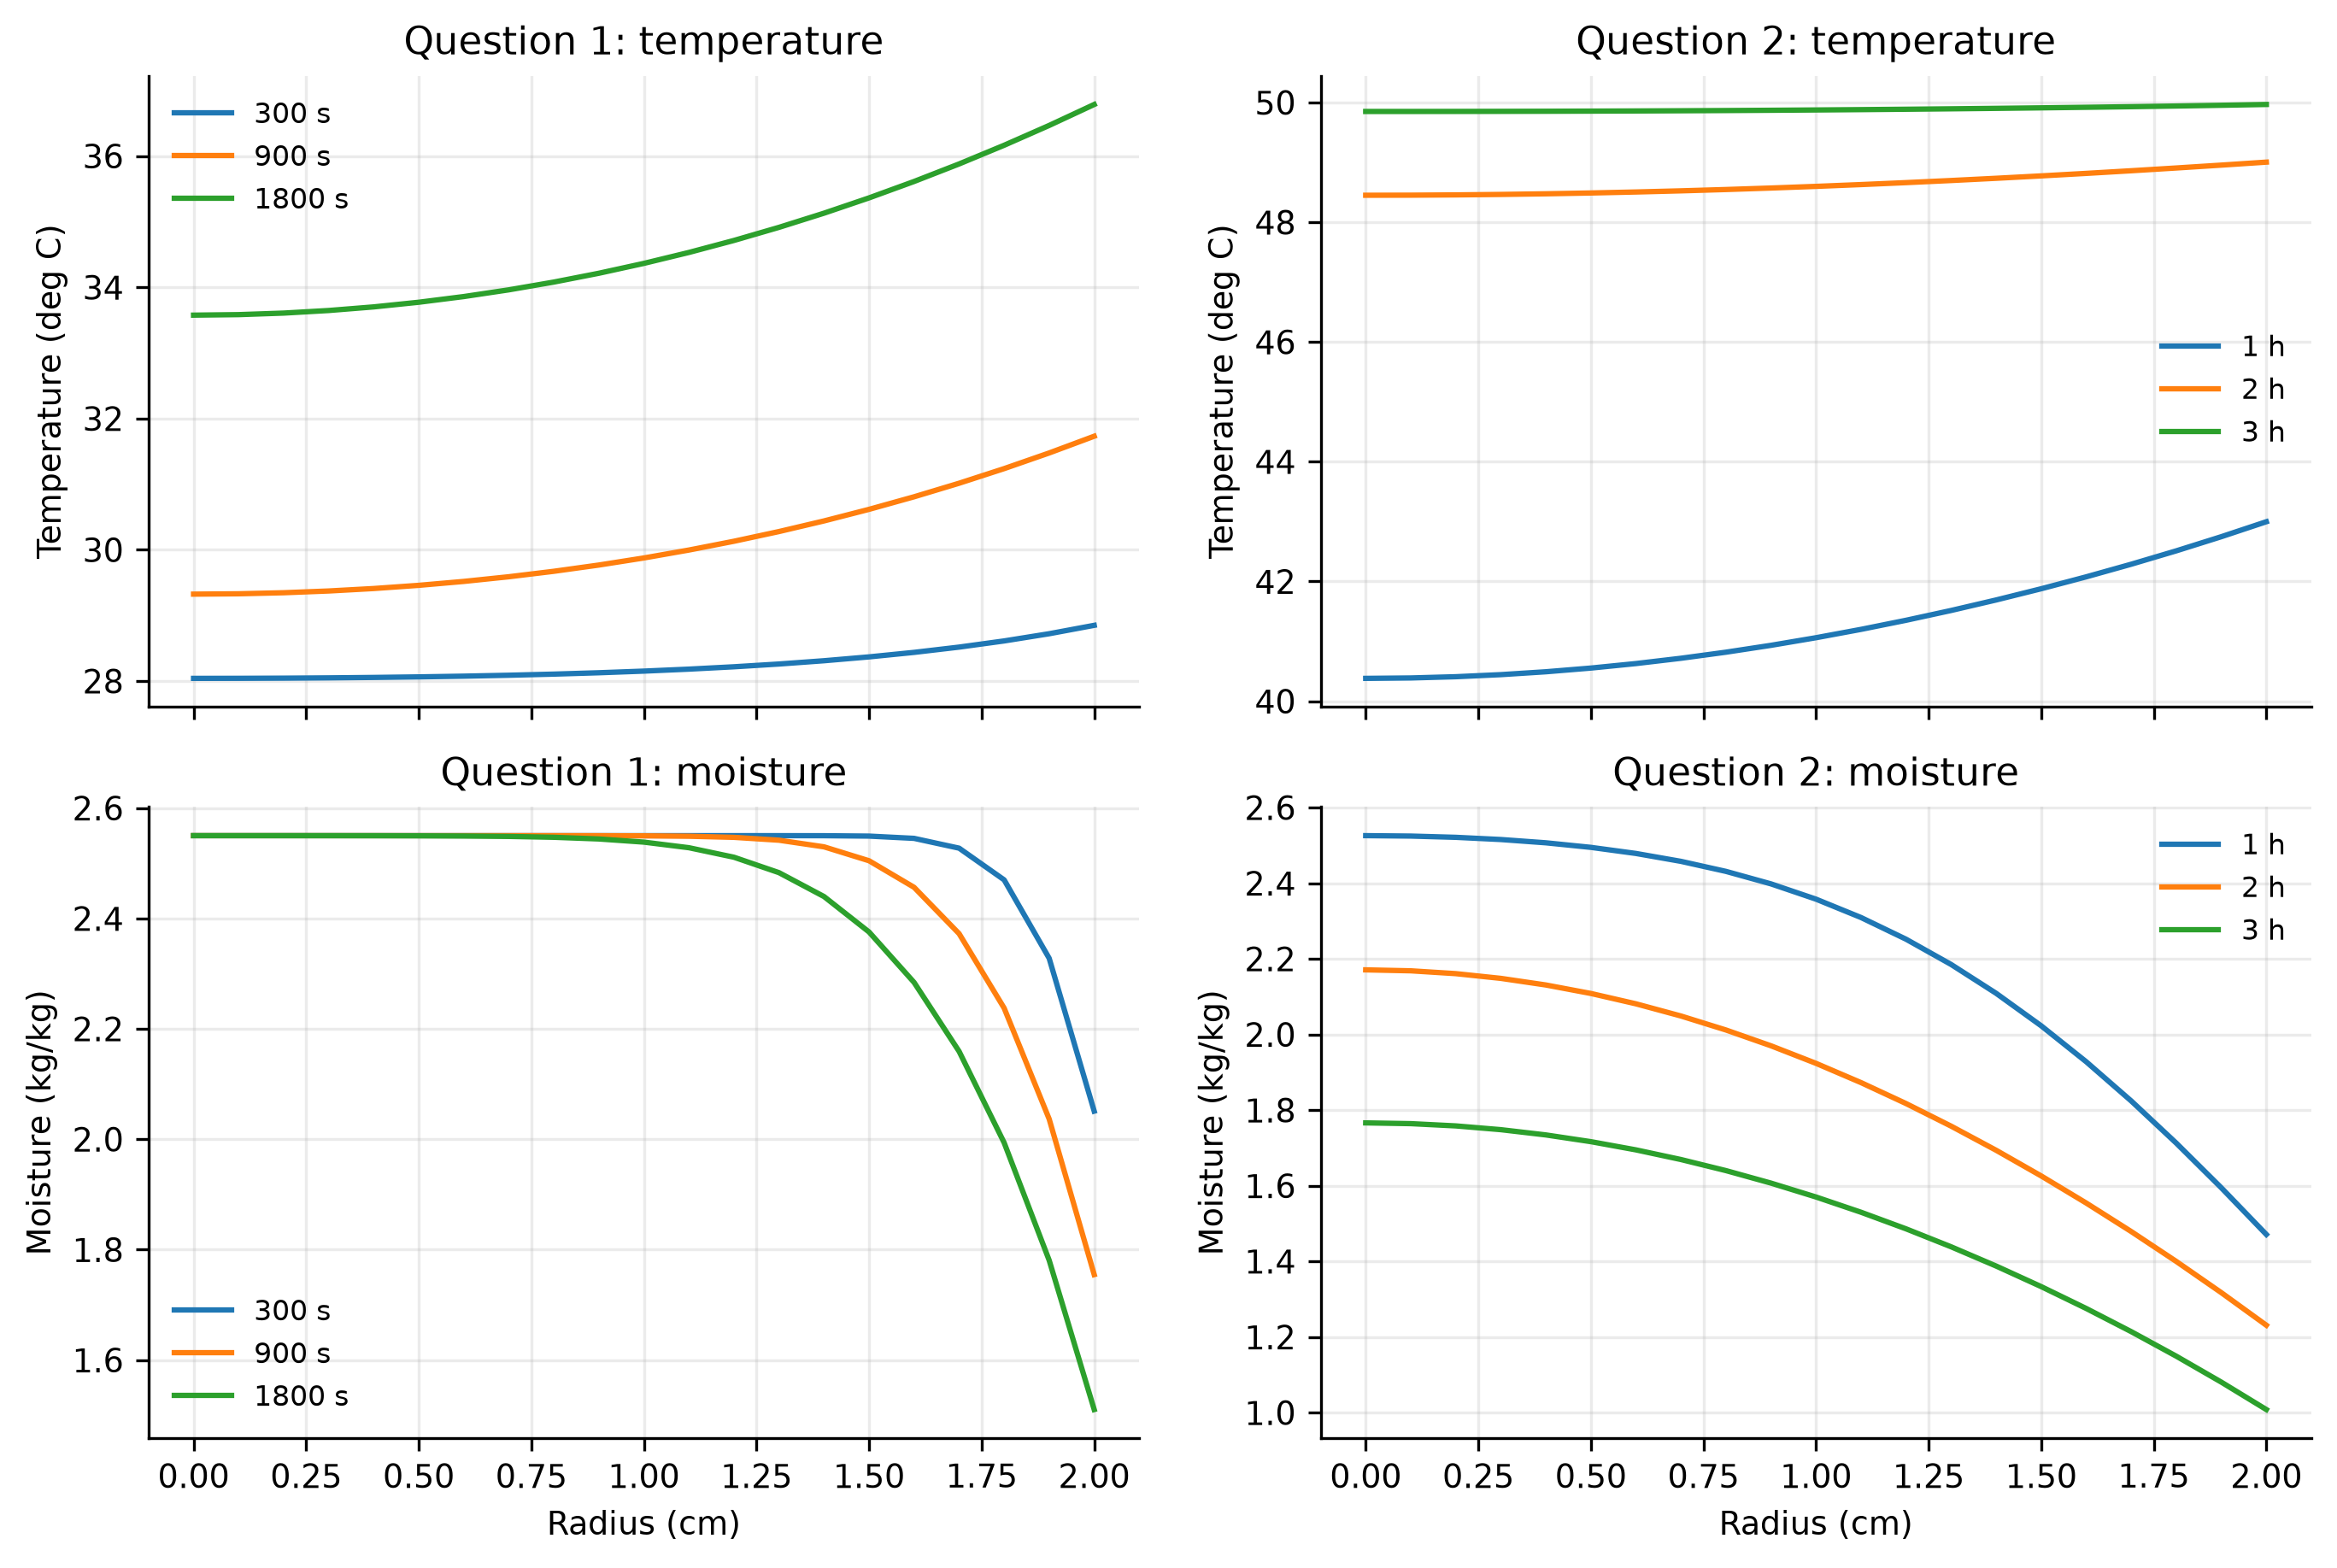
\includegraphics[width=0.94\textwidth]{early_profiles.png}
\caption{问题1和问题2的典型径向温湿剖面}\label{fig:profiles}
\end{figure}

\subsection{问题2：变物性条件下的前三小时}
问题2中，$D(C,T)$ 随升温增大、随含水率降低而显著减小。10800 s时中心和表面温度分别为49.8495 $^\circ$C与49.9664 $^\circ$C，径向温差已经很小；中心和表面含水率分别为1.7662 kg/kg与1.0081 kg/kg，仍保持较强梯度。说明传热时间尺度远短于传质时间尺度，但长期求解仍需保留温度对扩散系数的作用。

\subsection{问题3：固定半径的烘干时长}
沿用问题2模型并监测全场最大含水率，得到
\[
\boxed{t_3=\QThreeDryHours\ \mathrm h=2.3971\ \mathrm d}.
\]
中心始终是含水率最大处，也是最后达标位置。图\ref{fig:drying}表明，表面含水率约在12 h附近已低于阈值，而中心仍需约45 h；若以表面或平均含水率判停，将显著低估烘干时长。
\begin{figure}[H]
\centering
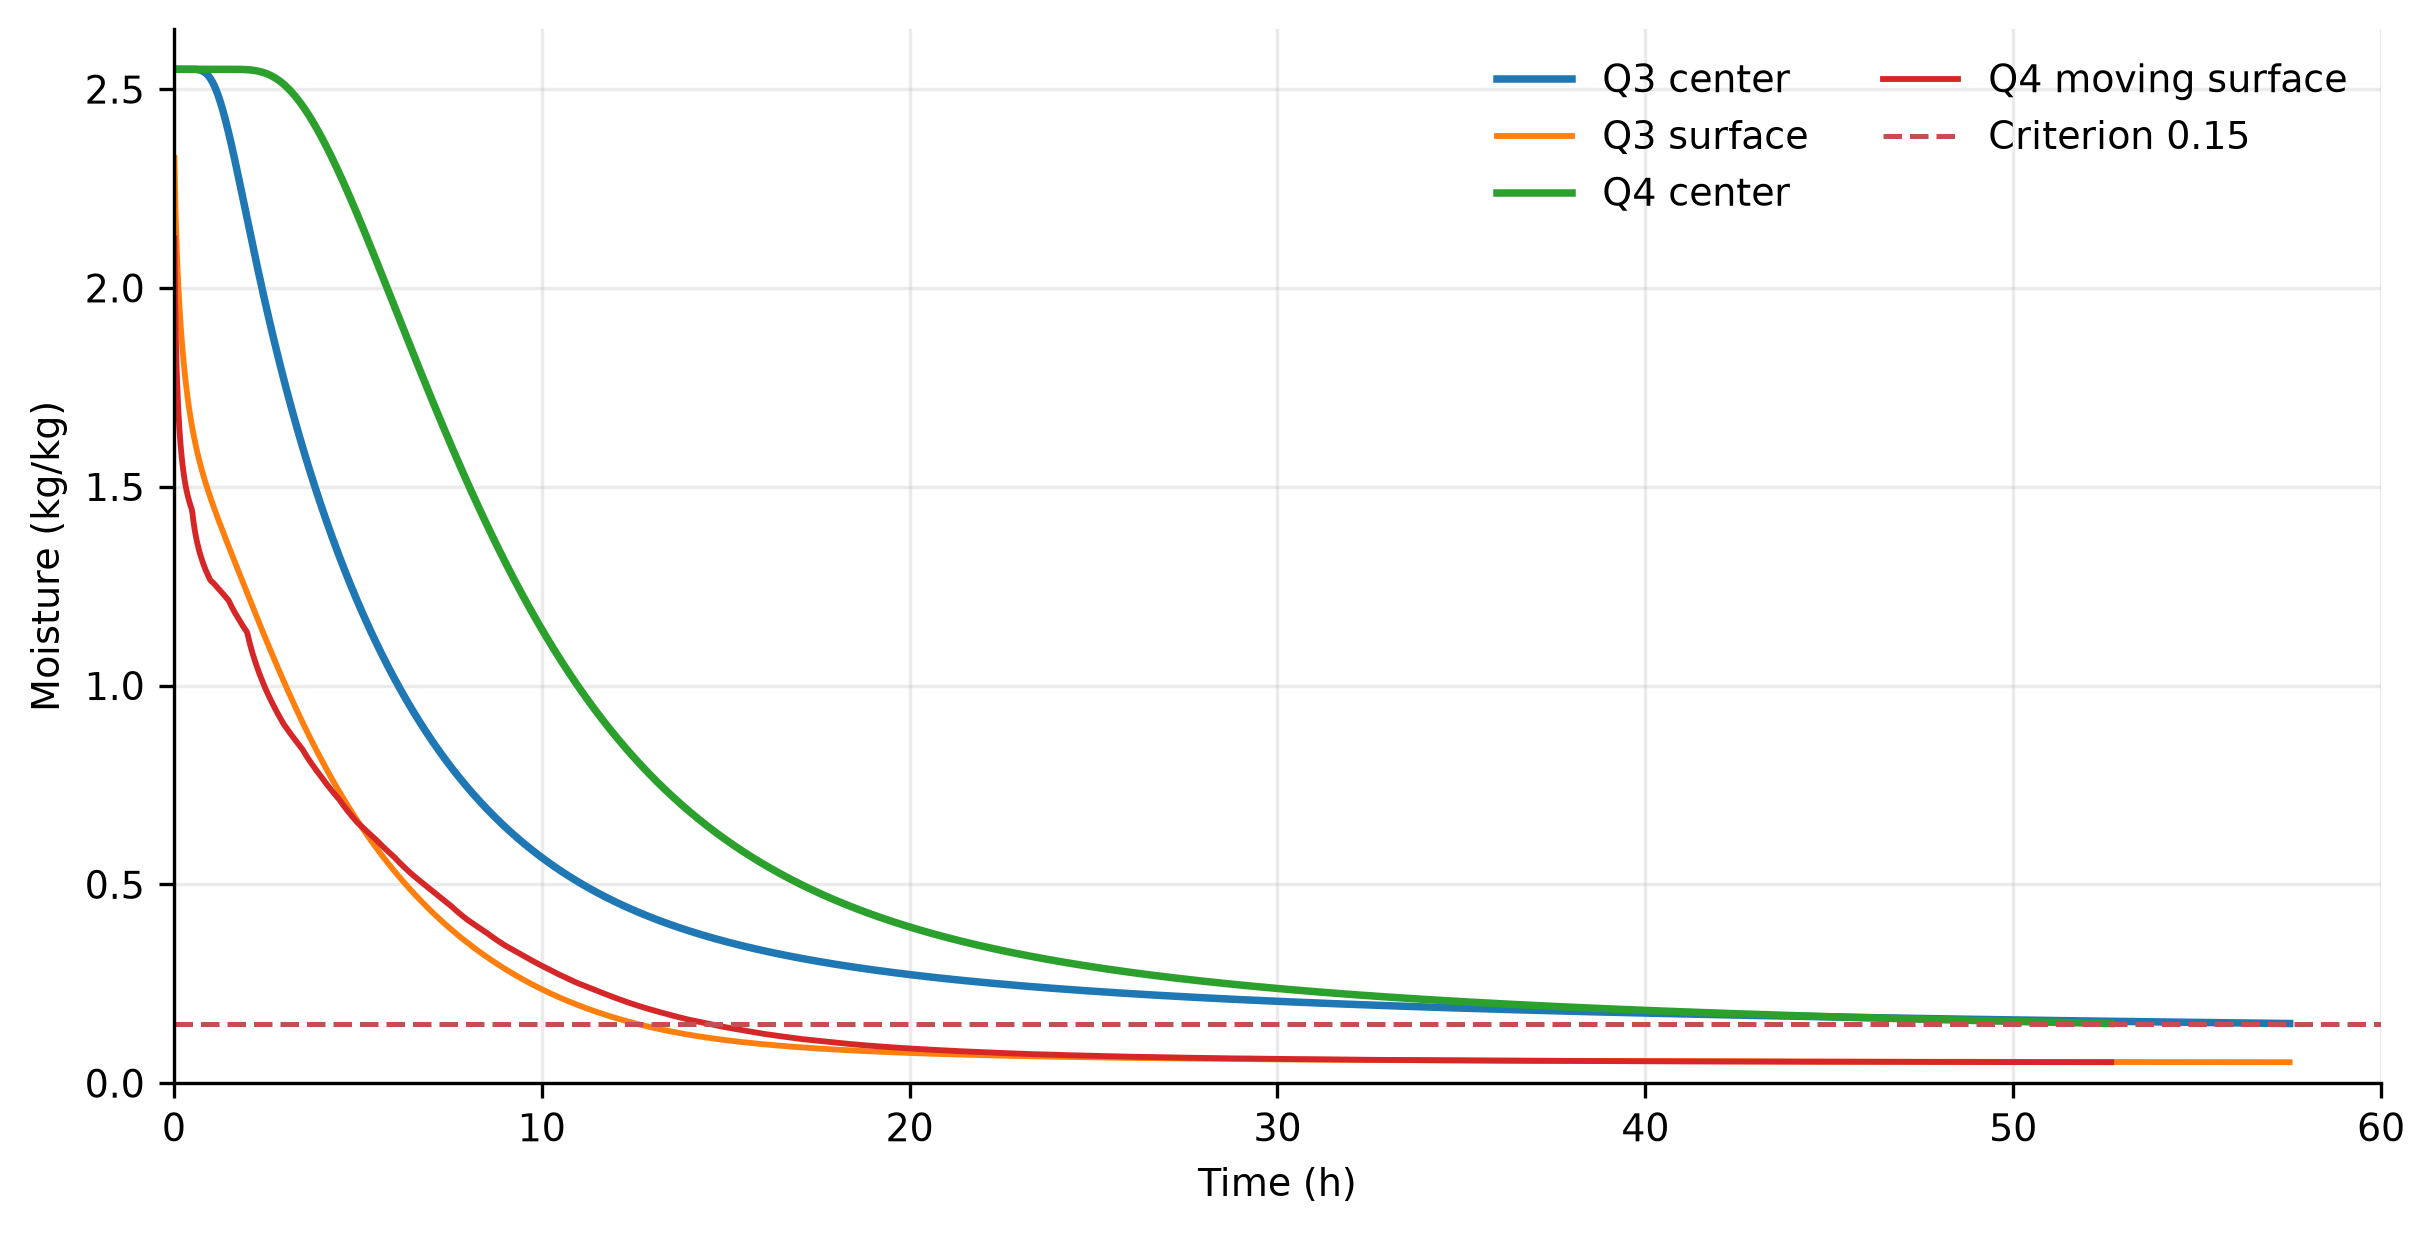
\includegraphics[width=0.90\textwidth]{drying_curves.png}
\caption{问题3与问题4中心和表面含水率演化}\label{fig:drying}
\end{figure}

\subsection{问题4：收缩条件下的烘干时长}
使用附录4物性、附件2的 $R(t)$ 和式\eqref{eq:movingT}--\eqref{eq:movingC}，得到
\[
\boxed{t_4=\QFourDryHours\ \mathrm h=2.1949\ \mathrm d},
\qquad R(t_4)=\QFourDryRadius\ \mathrm{cm}.
\]
问题4仍由中心控制终止。输出固定物理位置 $r_j$ 时，先计算 $\xi_j=r_j/R(t)$ 并对 $C(\xi,t)$ 插值；若 $r_j>R(t)$，该位置已在药材外，故表6和 \texttt{result4.xlsx} 对应单元格留空，而“药材表面”始终取 $\xi=1$。

为区分物性和几何效应，设置四个对照：附录3、固定2 cm时为\QThreeDryHours\ h；仅改用附录4而不收缩时为\AppendixFourFixedHours\ h；附录4并考虑完整收缩时为\QFourDryHours\ h；省略几何输运项时为\NoCoordinateCaseHours\ h。附录4物性在固定半径下使时长增加\AppendixIncrease；在同为附录4时，实测收缩使时长减少\ShrinkReduction。省略几何输运项会低估问题4时长约2.97\%，因此不能作为主结果。

\subsection{题目规定的结果表}
以下六表由最终计算数组自动生成，数值保留四位小数；完整逐秒或逐分钟数据见支撑文件。
\begin{table}[H]
\centering
\caption{问题1：30 min 内药材温度（$^\circ$C）}\label{tab:q1t}
\small
\begin{tabular}{rrrrrr}
\toprule
时间/s & 0 cm & 0.5 cm & 1.0 cm & 1.5 cm & 2.0 cm \\
\midrule
100 & 28.0001 & 28.0003 & 28.0041 & 28.0327 & 28.1801 \\
300 & 28.0408 & 28.0635 & 28.1514 & 28.3681 & 28.8489 \\
600 & 28.4533 & 28.5360 & 28.8039 & 29.3159 & 30.1652 \\
900 & 29.3243 & 29.4583 & 29.8755 & 30.6161 & 31.7304 \\
1200 & 30.5427 & 30.7098 & 31.2223 & 32.1126 & 33.4276 \\
1500 & 31.9957 & 32.1867 & 32.7660 & 33.7463 & 35.1203 \\
1800 & 33.5753 & 33.7720 & 34.3642 & 35.3621 & 36.7856 \\
\bottomrule
\end{tabular}
\end{table}

\begin{table}[H]
\centering
\caption{问题1：30 min 内水分浓度（kg/kg）}\label{tab:q1c}
\small
\begin{tabular}{rrrrrr}
\toprule
时间/s & 0 cm & 0.5 cm & 1.0 cm & 1.5 cm & 2.0 cm \\
\midrule
100 & 2.5500 & 2.5500 & 2.5500 & 2.5500 & 2.2471 \\
300 & 2.5500 & 2.5500 & 2.5500 & 2.5492 & 2.0508 \\
600 & 2.5500 & 2.5500 & 2.5500 & 2.5353 & 1.8770 \\
900 & 2.5500 & 2.5500 & 2.5497 & 2.5045 & 1.7547 \\
1200 & 2.5500 & 2.5500 & 2.5482 & 2.4646 & 1.6586 \\
1500 & 2.5500 & 2.5499 & 2.5445 & 2.4206 & 1.5787 \\
1800 & 2.5500 & 2.5497 & 2.5383 & 2.3755 & 1.5102 \\
\bottomrule
\end{tabular}
\end{table}

\begin{table}[H]
\centering
\caption{问题2：3 h 内药材温度（$^\circ$C）}\label{tab:q2t}
\small
\begin{tabular}{rrrrrr}
\toprule
时间/h & 0 cm & 0.5 cm & 1.0 cm & 1.5 cm & 2.0 cm \\
\midrule
0.5 & 32.1892 & 32.3821 & 32.9659 & 33.9608 & 35.4130 \\
1.0 & 40.3816 & 40.5536 & 41.0605 & 41.8782 & 42.9976 \\
1.5 & 45.8468 & 45.9348 & 46.1930 & 46.6051 & 47.1401 \\
2.0 & 48.4502 & 48.4881 & 48.5984 & 48.7736 & 49.0033 \\
2.5 & 49.4670 & 49.4792 & 49.5137 & 49.5653 & 49.6609 \\
3.0 & 49.8495 & 49.8553 & 49.8746 & 49.9101 & 49.9664 \\
\bottomrule
\end{tabular}
\end{table}

\begin{table}[H]
\centering
\caption{问题2：3 h 内水分浓度（kg/kg）}\label{tab:q2c}
\small
\begin{tabular}{rrrrrr}
\toprule
时间/h & 0 cm & 0.5 cm & 1.0 cm & 1.5 cm & 2.0 cm \\
\midrule
0.5 & 2.5499 & 2.5489 & 2.5256 & 2.3257 & 1.6486 \\
1.0 & 2.5257 & 2.4948 & 2.3578 & 2.0230 & 1.4711 \\
1.5 & 2.3861 & 2.3256 & 2.1344 & 1.8020 & 1.3476 \\
2.0 & 2.1709 & 2.1084 & 1.9236 & 1.6259 & 1.2311 \\
2.5 & 1.9566 & 1.9006 & 1.7360 & 1.4720 & 1.1166 \\
3.0 & 1.7662 & 1.7165 & 1.5702 & 1.3333 & 1.0081 \\
\bottomrule
\end{tabular}
\end{table}

\begin{longtable}{rrrrrr}
\caption{问题3每6 h及达标时刻的水分浓度}\label{tab:q3}\\
\toprule
时间/h & 0 cm & 0.5 cm & 1.0 cm & 1.5 cm & 2.0 cm \\
\midrule
\endfirsthead
\toprule
时间/h & 0 cm & 0.5 cm & 1.0 cm & 1.5 cm & 2.0 cm \\
\midrule
\endhead
6 & 1.0169 & 0.9881 & 0.9015 & 0.7550 & 0.5328 \\
12 & 0.4561 & 0.4431 & 0.4030 & 0.3297 & 0.1642 \\
18 & 0.2988 & 0.2915 & 0.2687 & 0.2253 & 0.0844 \\
24 & 0.2378 & 0.2327 & 0.2167 & 0.1856 & 0.0664 \\
30 & 0.2058 & 0.2019 & 0.1892 & 0.1642 & 0.0598 \\
36 & 0.1859 & 0.1826 & 0.1719 & 0.1505 & 0.0566 \\
42 & 0.1721 & 0.1692 & 0.1598 & 0.1408 & 0.0548 \\
48 & 0.1619 & 0.1592 & 0.1508 & 0.1336 & 0.0537 \\
54 & 0.1539 & 0.1515 & 0.1437 & 0.1278 & 0.0530 \\
57.5303 & 0.1500 & 0.1477 & 0.1402 & 0.1250 & 0.0527 \\
\bottomrule
\end{longtable}

\begin{longtable}{rrrrrr}
\caption{问题4每6 h及达标时刻的水分浓度}\label{tab:q4}\\
\toprule
时间/h & 半径/cm & 0 cm & 0.5 cm & 1.0 cm & 药材表面 \\
\midrule
\endfirsthead
\toprule
时间/h & 半径/cm & 0 cm & 0.5 cm & 1.0 cm & 药材表面 \\
\midrule
\endhead
6 & 1.3740 & 1.9530 & 1.7835 & 1.2579 & 0.5678 \\
12 & 1.2480 & 0.8738 & 0.7767 & 0.4862 & 0.2147 \\
18 & 1.2140 & 0.4594 & 0.4131 & 0.2653 & 0.1021 \\
24 & 1.2040 & 0.3072 & 0.2806 & 0.1903 & 0.0714 \\
30 & 1.2010 & 0.2381 & 0.2199 & 0.1556 & 0.0610 \\
36 & 1.2000 & 0.2000 & 0.1861 & 0.1357 & 0.0567 \\
42 & 1.2000 & 0.1761 & 0.1648 & 0.1228 & 0.0545 \\
48 & 1.2000 & 0.1597 & 0.1500 & 0.1136 & 0.0533 \\
52.6776 & 1.2000 & 0.1500 & 0.1413 & 0.1081 & 0.0526 \\
\bottomrule
\end{longtable}


\subsection{数值验证与可行性分析}
粗网格会高估干燥时间，问题3尤其明显，因为低含水率时 $D$ 指数下降并形成薄低扩散层。问题3由641加密到1281个 $r$ 节点，时长变化仅\QThreeGridChange；问题4由321加密到641个 $\xi$ 节点，变化仅\QFourGridChange；问题4把时间步由30 s减至15 s，变化为\QFourTimeChange。收敛曲线见图\ref{fig:grid}。
\begin{figure}[H]
\centering
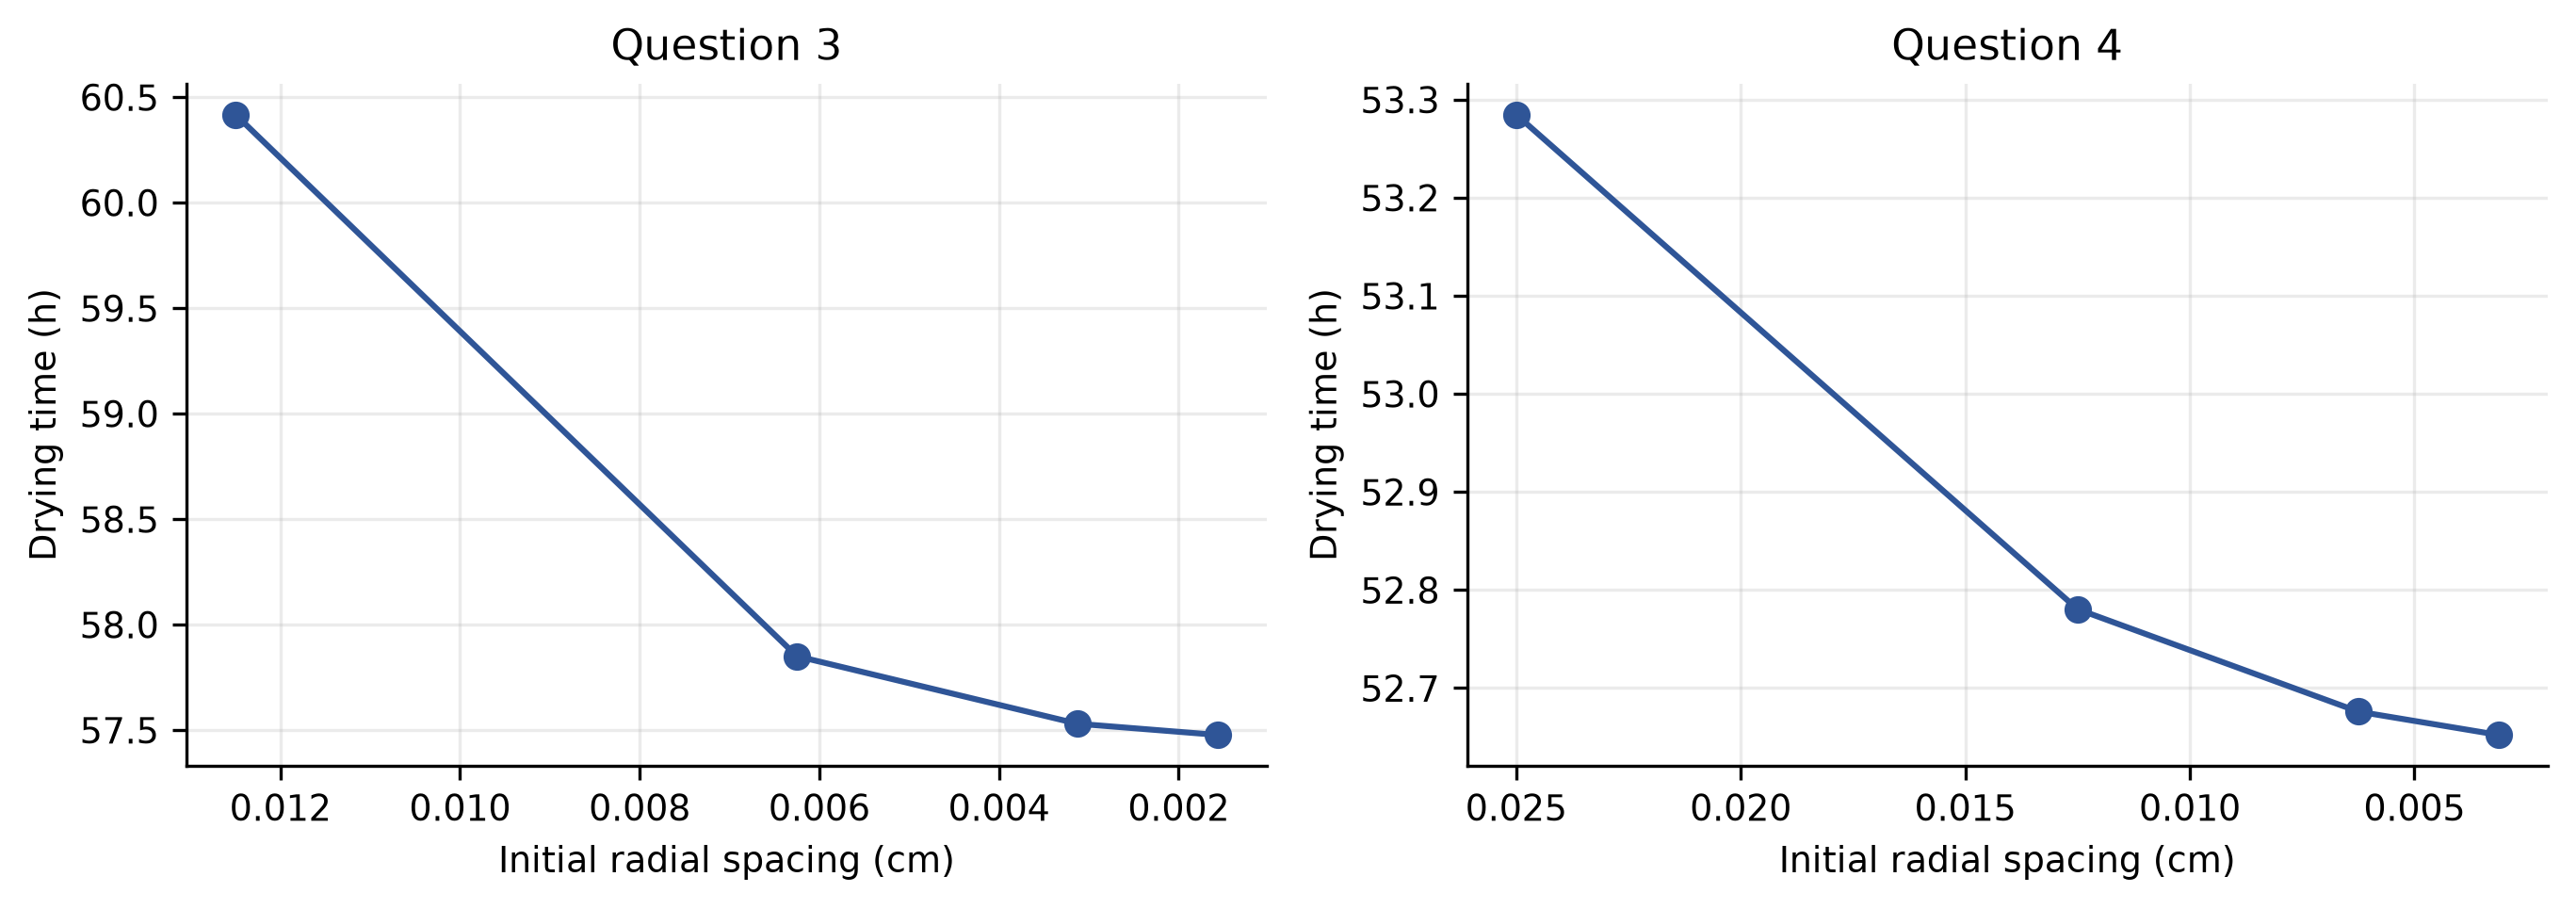
\includegraphics[width=0.94\textwidth]{grid_convergence.png}
\caption{问题3、4的空间网格收敛}\label{fig:grid}
\end{figure}
\begin{table}[H]
\centering
\caption{干燥时长的空间收敛数据}
\begin{tabular}{rrr@{\hspace{2em}}rrr}
\toprule
\multicolumn{3}{c}{问题3：划分 $r$} & \multicolumn{3}{c}{问题4：划分 $\xi$}\\
节点数 & $\Delta r$/cm & 时长/h & 节点数 & 初始间距/cm & 时长/h\\
\midrule
161  & 0.012500 & 60.4179 & 81  & 0.025000 & 53.2848\\
321  & 0.006250 & 57.8506 & 161 & 0.012500 & 52.7805\\
641  & 0.003125 & 57.5302 & 321 & 0.006250 & 52.6760\\
1281 & 0.001563 & 57.4771 & 641 & 0.003125 & 52.6522\\
\bottomrule
\end{tabular}
\end{table}

令 $h=h_m=0$ 并从非均匀含水率初值计算1 h，按 $r$ 区间积分权重求得的总水分相对变化为\ConservationError，验证了相邻界面通量的抵消。令初值与恒定环境完全相同，600 s后温度、含水率最大绝对误差为\EquilibriumError，验证了边界符号。问题1、2中321与641节点在规定表格位置的含水率最大差分别为\QOneMoistureProfileError、\QTwoMoistureProfileError，温度差均小于 $6\times10^{-6}$ $^\circ$C。所有正式算例无负含水率，温度均在初值与环境边界构成的范围内，且问题4终点早于附件2的72 h数据上限。因此所得数值在守恒性、收敛性和物理方向上均可行。

\section{模型总结}
\subsection{主要结论}
一维圆柱径向热质耦合模型能够统一处理四个问题。问题3的全域达标时间为\QThreeDryHours\ h，问题4完整移动边界模型为\QFourDryHours\ h。收缩把附录4固定半径情况下的\AppendixFourFixedHours\ h显著降至约52.68 h，说明扩散距离是决定烘干效率的关键几何因素。全过程均由中心最后达到含水率阈值。

\subsection{模型优点}
\begin{enumerate}
  \item 四问共享同一热质传递框架，仅替换物性、半径模型和终止事件。
  \item 离散符号与物理坐标一致：问题1--3划分 $r$，问题4划分 $\xi$；半节点区间的守恒积分同时处理圆心、Robin边界和通量抵消。
  \item 计算网格与输出网格分离，并以空间收敛、时间收敛、封闭系统守恒和平衡态检验确定精度。
  \item 移动边界同时保留 $R^{-2}$ 与 $\xi\dot R/R$ 项，并定量评估了遗漏几何输运项的影响。
\end{enumerate}

\subsection{局限与改进}
模型未显式描述蒸发潜热、表面平衡含水率、轴向传递和长度收缩；问题2--4的 $h,h_m$ 只能沿用题目给定值。附件2提供的是半径历史而非收缩本构，因此问题4属于实测几何驱动模型。若获得独立实验曲线，可进一步反演 $h_m$ 和平衡含水率关系，建立 $R(C)$ 收缩本构，并用守恒型任意拉格朗日--欧拉格式及二维轴对称模型复核几何项与端部效应。

\subsection{支撑文件与复现}
支撑材料包括 \texttt{src/drying\_solver.py}、\texttt{run\_all.py}、\texttt{validate\_results.py}、自动生成图表和Excel的工具脚本，以及四个结果工作簿。算法依次读取附件、建立 $r$ 或 $\xi$ 网格、隐式推进并Picard迭代、检查终止事件，最后将精细网格结果插值到题目规定时间和位置。详细命令、参数和文件结构见随附代码说明书。

\begin{thebibliography}{9}
\bibitem{crank} Crank J. \textit{The Mathematics of Diffusion}. 2nd ed. Oxford: Clarendon Press, 1975.
\bibitem{patankar} Patankar S V. \textit{Numerical Heat Transfer and Fluid Flow}. New York: Hemisphere, 1980.
\bibitem{hairer} Hairer E, Wanner G. \textit{Solving Ordinary Differential Equations II: Stiff and Differential-Algebraic Problems}. 2nd ed. Berlin: Springer, 1996.
\bibitem{incropera} Incropera F P, DeWitt D P, Bergman T L, Lavine A S. \textit{Fundamentals of Heat and Mass Transfer}. 6th ed. Hoboken: Wiley, 2007.
\bibitem{mujumdar} Mujumdar A S, ed. \textit{Handbook of Industrial Drying}. 4th ed. Boca Raton: CRC Press, 2014.
\end{thebibliography}

\end{document}
